% icstdoc.tex V1.11 11 April 2011
%brave new ideas, artistic installations with technological content, technical creative demonstrators
\documentclass[fonts]{icst}

\usepackage{moreverb}

\usepackage[breaklinks,colorlinks,bookmarksopen,bookmarksnumbered,linkcolor=ICSTblue,citecolor=ICSTblue,urlcolor=ICSTblue]{hyperref}
\usepackage{breakurl}
\usepackage{doi}
\usepackage{float}
\usepackage{graphicx}


\newcommand\BibTeX{{\rmfamily B\kern-.05em \textsc{i\kern-.025em b}\kern-.08em
T\kern-.1667em\lower.7ex\hbox{E}\kern-.125emX}}

\def\volumeyear{2014}

\begin{document}

\runningheads{Tomazic, Tomaz; Lai Chin Chung, Louis}{Trzaska cesta 25, 1000 Ljubljana}

\title{Virtual Skiing}

\author{Tomazic, Tomaz; Lai Chin Chung, Louis}

\address{University of Ljubljana, Faculty of informatics and computer science}

\abstract{This paper describes a virtual skiing game using kinect and unity 3D.}

\keywords{skiing, kincect, unity 3D, virtual}


\maketitle

\section{Introduction}
The interactive installation "Virtual skiing" enables a visual immersion into the feelings of gliding on snow through a winter landscape. The computer rendered winter landscape is displayed over the entire wall in front of the skier. As on real skis you can regulate the speed of descent by changing the posture of your body so that the air resistance is decreased or increased. By shifting the weight of your body to the right or left ski you can make turns down the slope between the snow capped trees. The interface to the virtual world is implemented by computer vision techniques which capture the posture of the skier's body. \cite{ORIG}).

\section{Software overview}
\subsection{Goal of the project}
The goal of the project is to provide the user a virtual skiing experience. To do so, at least the following needs to be done:
\begin{enumerate}
\item[(i)] track body movement of the user
\item[(ii)] display a virtual 3D environment on a screen
\item[(iii)] play game in this enviroment
\end{enumerate}


\subsection{Kinect}
\subsubsection{Overview}
Kinect is the most convienent body movement tracking hardware we can find in the market, it thus becomes the tool for our project. The Kinect sensor haveo one RGB camera and two Infra-red sensors, allowing it to track movement to/from any direction in a 3D space. 

\subsubsection{Code}
By examining the sample code, a skeleton of user is made using C\#. A skeleton consist of nodes and lines, nodes representing the the joints of the user, lines representing the limbs/body of the user. By comparing the positions nodes, we can capture the user's movement and turn them into inputs in the game.There are 2 main types of input in the skiing game, one controls the direction and the other controls the speed of skiing.

\subsubsection{Directions}
To control the direction of ski, user need to band their body left or right to turn, or stay in the middle to go straight. A simple method is used to extract this particular movement by the user, we simply compare the nodes on both shoulders. The data obtained is then threasholded into only 3 inputs, left, middle and right. 

\subsubsection{Speed}
The user need to squat to increase the speed, and detection of squatting is needed. When squatting, the position of the node on hip is changing obviously. So, the node on hip is used to determine whether the user is squatting or not.

\subsection{Unity 3D}
Unity is a development engine for the creation of 2D and 3D games and interactive content. It has multiplatform support and own asset store where you can download scripts, objects, scenes.. \cite{UNITY}

\subsubsection{Terrain}
It has great support for creating terrain. In game we created simple terrain with mountains and put snow on it. For more flexible terrain we could create scirpt or just few images of pre-difined heightmaps. Unity have option to generate terrain using hightmap.
\subsubsection{Scripting}
Unity support C\#, javascript and Boo scripting languages. It also supports applying different languaged script on same object. We used such ability for user movement in skiing game, using javascript and C\# languages only.

\section{Developing process}
\subsection{Planning}
\subsubsection{Mindmap}
A mindmap is made to record all the ideas about the project. It gives the team some guide and direction to work on. This is also the step where we know each team member's strength and weakness, leads to better allocation of work later on. 

\begin{figure}
    \centering
    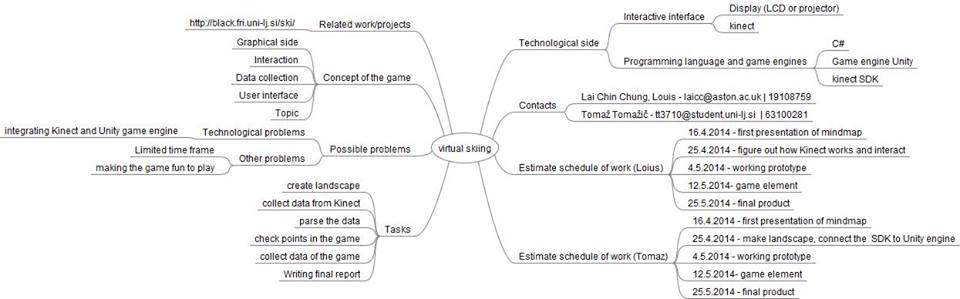
\includegraphics[width=0.4\textwidth]{mindmap.png}
    \caption{Mindmap}
    \label{fig:awesome_image}
\end{figure}

\subsection{Research}
\subsubsection{Kinect}
At the beginning of the project, none of the team member knows anything about programming on Kinect, it is the main focus of search. We found that Kinect SDK is essential in coding the sensor, it comes together with Kinect studio and a developer toolkit. Kinect studio is just for testing and the developer toolkit is a package of code examples.

\subsubsection{Game engine}
It took us almost no time to search for game engine, one of the team member knows how to use Unity 3D, certainly this becomes your choice of game engine. 

\subsubsection{Designing the system}

\subsection{Work on the project}

\begin{figure}
    \centering
    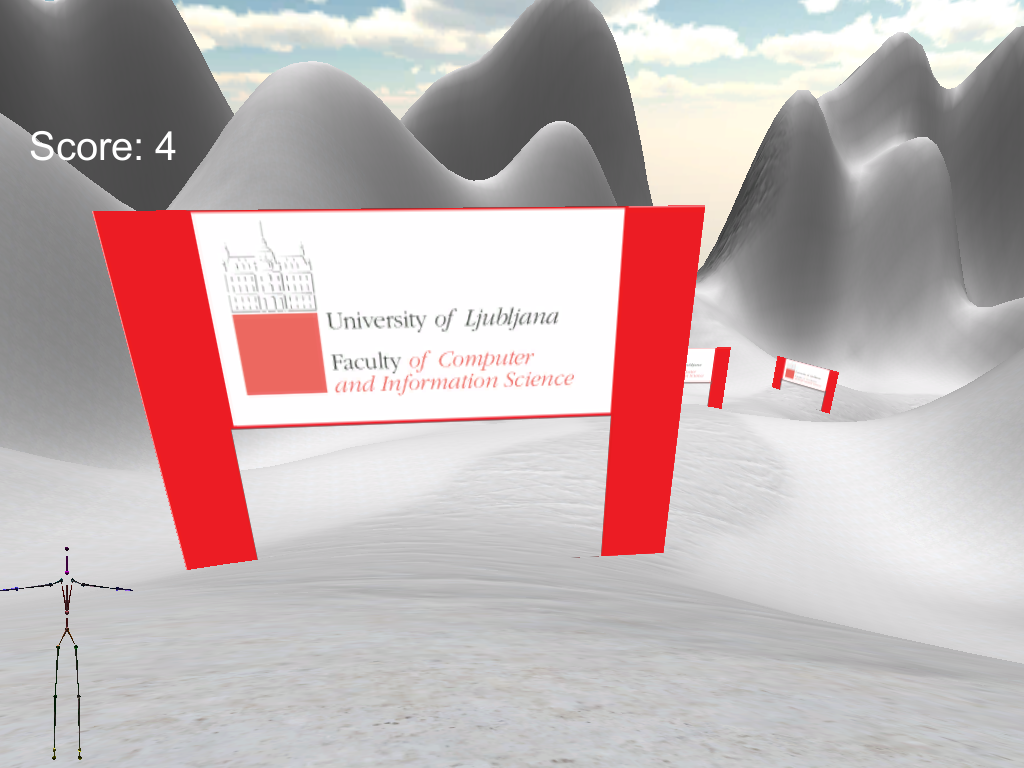
\includegraphics[width=0.4\textwidth]{game.png}
    \caption{Screenshot form skiing game.}
    \label{fig:awesome_image}
\end{figure}

\subsection{Replanning}

\subsection{Ending}

\section{Conclusions}

\subsection{Schedule (planned vs read)}
a

sub


\begin{thebibliography}{9}

\bibitem{ORIG} \textsc{Solina Franc} and \textsc{Batagelj Borut} (2005) \emph{http://black.fri.uni-lj.si/ski/}

\bibitem{UNITY} \textsc{Unity 3D} (2014) \emph{\LaTeX: \url{http://docs.unity3d.com/ScriptReference/index.html}}

\end{thebibliography}
\end{document}
